\documentclass[10pt,a4paper]{article}
\usepackage[utf8]{inputenc}
\usepackage{amsmath}
\usepackage{amsfonts}
\usepackage{amssymb}
\usepackage{a4wide} %Wider margins
\usepackage[english]{babel} %English dictionary for hyphenation and definitions, e.g. Table vs. Tabel
\usepackage[official]{eurosym} %Support for Euro-sign
\usepackage[utf8]{inputenc} %Support for internationalization, e.g. é vs.\’e
\usepackage{amsmath,amssymb,amsthm} %Support for mathematical formulas and symbols
\usepackage{fancyhdr} %Fancy headers
\usepackage{hyperref} %Creates clickable links
\usepackage{graphicx} %Support for grahpics
\usepackage{nopageno} %Support for removal of pagenumbers
\usepackage{tabularx}
\usepackage{enumitem}
\usepackage{xspace}
\usepackage{algorithm,algpseudocode}
\usepackage{float}
\usepackage{mathtools}
\usepackage[dvipsnames]{xcolor}
\usepackage[titletoc,toc,title]{appendix}
\usepackage{listings}
\usepackage{makecell}
\graphicspath{ {./ThesisFigures/} }

\hypersetup{
    pdftitle={}, %PDF-file will be given a proper title when viewed in a reader
    hidelinks %PDF-file will be given clickable, yet not visible links when viewed in a reader
}
\newcommand{\documenttitle}{TPOT's performance for Biomedical Data}
\newcommand{\documentsubtitle}{A Data Mining Seminar}


\newcommand{\true}{{\sc True}\xspace}
\begin{document}
	
	\begin{titlepage}
		
		\center
		
		\vspace*{3cm}
		
		\textbf{\huge \documenttitle}
		
		\textit{\LARGE \documentsubtitle}
		
		\vspace*{2cm}
		
		\large
		\centering
		T.P.A.~\textsc{Beishuizen}~(0791613)\\
		Biomedical Engineering - Computational Biology\\
		Data Engineering - Information Systems\\
		Eindhoven, University of Technology\\
		Email: \texttt{t.p.a.beishuizen@student.tue.nl}
		
		\vfill
		
		\vspace*{1cm}
		
		\today
		
	\end{titlepage}
	
	\tableofcontents
	
	%\newpage
	
	\pagestyle{fancy}
	%Abbreviations used by fancyhdr:
	%E Even page
	%O Odd page
	%L Left field
	%C Center field
	%R Right field
	%H Header
	%F Footer
	\fancyhead{} % clear all header fields
	\fancyfoot{} % clear all footer fields
	\renewcommand{\headrulewidth}{0.4pt}
	\renewcommand{\footrulewidth}{0.4pt}
	
	\fancyhead[L]{\rightmark}
	\fancyfoot[C]{\thepage}
	\fancyhead[R]{T.P.A. Beishuizen}
	
	
	\clearpage
	
	\section{Introduction}
	\label{sec:Introduction}
	
	% Quick explanation for biomedical data
	At the Computational Biology department (cBio) of Biomedical Engineering (BME), many requests are made to analyse gathered data. This data usually stems from research in hospitals, but can also be from other BME groups and publicly available data. Currently a standard is missing to efficiently analyse those data sets. With the vast number of data sets that are available, such a standard in the form of a framework on data analysis would be valuable. It would speed up projects and give them a higher chance to succeed the goal, due to improved efficiency.
	
	% Quick explanation bariatric data
	An example of biomedical data sets from cBio stemmed from the Catharina Hospital in Eindhoven. This extensive data set was a combination of two data sets. The first is a data set filled out by a doctor that analysed basic human features as well as the presence of co-morbidities. The second data set consisted of 41 markers measured pre- and post-surgery for 2367 patients that underwent gastric sleeve or gastric bypass surgery, also known as bariatric surgeries. The number of bariatric surgeries is increasing worldwide. Although initially thought otherwise, this type of surgery has added benefits on top of losing weight. Among those benefits the remission of metabolic co-morbidities can be named. Due to binary labelling of those co-morbidities, valuable information is lost. On top of that the labelling is not clearly defined either. To obtain more and better results, this binary labelling could be replaced by a continuous severity score. Ruben Deneer conducted a research on trying to achieve a successful replacement. This data set is a prime example of a data set that is not trivially preprocessed, when looking at multiple data sets, missing values and erroneous data.\cite{Deneer2017Thesis}
	
	% Quick explanation for automated machine learning
	A possible solution for partly providing a framework for cBio can be found in automated machine learning (autoML). This relatively new extension to machine learning tries to automatically search the best combination of preprocessing, feature selection and machine learning algorithms to efficiently describe a data set. CPU or actual time and memory usage are the two main constraints for autoML, due to testing different methods with varying parameters taking up time and space. These autoML algorithms usually are made with the combined algorithm selection and hyperparameter optimization (CASH) challenge in mind.\cite{feurer2015efficient} 
	
	% Introduction of TPOT
	Olson and Moore proposed a tool for autoML, a Tree-based Pipeline Optimization Tool (TPOT).\cite{olson2016tpot} This tool also tries to find the best classifier by creating pipelines for the different algorithms. The pipelines are evaluated and branched or altered according to the evaluation. It makes use of genetic programming, a technique used for evolutionary computations.\cite{banzhaf1998genetic} Evaluation of several TPOT approaches are proven better than doing a basic machine learning analysis and are therefore a promising approach for implementation. \cite{olson2016evaluation} Several projects used layering and meta-learning techniques to tackle the time and space constraints.\cite{Gijsbers2017Thesis}
	
	% TPOT and biomedical data
	To test if TPOT is also suitable for biomedical data, it must be tested by a specific set, such as the bariatric data set. This data consists of several biomedical data challenges only some of which seem solvable by TPOT. A research must be done to find out whether TPOT can manage to retrieve good results from this data set and may benefit of some improvements.
	
	% Layout data seminar
	For the data seminar, first the background will be given. This background will be about the biomedical data sets, the exemplary data set used for the seminar, a topic of automated machine learning and at last a part about TPOT. Secondly the research question is given, together with a hypothesis.
	
	\section{Background}
	\label{sec:Background}
	
	\subsection{Biomedical data}
	
	\label{subsec:BiomedicalData}
	
	% Biomedical engineering description.
	Biomedical engineering can be seen as a specific part of engineering with a wide variety of topics. These topics can be theoretical, non-experimental undertakings, but also state-of-the-art applications. Not only research and development can be used, but also implementation and operation. Combining all of these different parts in one definition is hard. \cite{bronzino2014biomedical} For this project, the focus is mainly on research and development, also known as knowledge discovery. \cite{bramer2007principles} 

	% Biomedical research summary
	When a biomedical engineer starts a project, at the start usually only a data set and the research goal are known. To achieve that certain goal from the data set, four aspects influence the project's course and development. At first obviously the data itself is a big part of such an influencer as the research is restricted to limitations from it. Examples of such restrictions are multidimensionality, set size, data heterogeneity, missing feature values and population handling. The other obvious influencer is the main research goal. Since the biomedical engineer wants to achieve a certain goal, the approach outcome must match that goal for the research to be successful. Most goals are focused around either data mining, extracting relations from available data, or modelling, creating a model within data features. A third influencer is the availability of data analysis tools. The steps to take from data to goal do not only include an approach, but also a tool to execute it. The choice of a certain tool has a big impact on the project, as each one of them has its own advantages and disadvantages. The two most well known tools within BME are MATLAB and Python, however some engineers have used R, Java or C++ and there are still other possibilities. A last big influencer is the biomedical knowledge. What experience the scientist already has with similar projects can greatly influence the choice of approach and framework. Knowledge of the supervisor and publicly known information on the research subject from books and articles also influence the approach, as already known outcomes do not have to be researched again. 
	
	% Process steps for biomedical research
	For data engineers the main focus lies in trying to find patterns in the data. Therefore in this seminar the focus will mainly be on the data driven aspect of a biomedical project. Characteristics of such a data driven approach (as mentioned before) are mainly focused around data volume, dimensionality, complexity, heterogeneity and quality.\cite{chen2006medical, doi:10.1093/bib/bbx044}
	
	% Volume challenge
	Collecting data because it is possible can make data sets bigger than needed. Both in number of instances and features, data sets can be harder to understand or analyse when more is available.\cite{chen2006medical} This volume problem usually is tackled by taking sub-populations of the complete set. These sub-sets can either be focused around a part of the population (gender, age, race) or taken at random to still represent all of it. Due to the efficiency of analysis techniques and the rise in computational speed of servers\cite{blythe2008rise}, volume on its own becomes less of an issue. Volume does however become an issue when combining with heterogeneity and quality. \cite{Turkay2014, Holzinger2014} 
	
	% Dimensionality challenge
	Not all data sets have a high number of instances that cause a big data volume. Sometimes there are relatively few instances, while the number of features is proportionally high. \cite{dubitzky2007fundamentals} Usually many of those features are not relevant enough for the research, however are still used for testing. Trying to remove features that are not important, will greatly help finding relations between the others and create more knowledge about the research topic. Lowering the number of features also makes the data volume go down, so analysis should be easier. Mainly an optimal features set should be selected to obtain the best results. \cite{PENG201015}
	
	% Complexity challenge
	Biomedical data can also be very complex. Useful results may be present, however it can be very hard to obtain it. Examples of complex data are images, several biomedical signals and temporal data. Details of the useful results that are present in images can for example be very hard to detect, the temporal data can vary quite much over time and the biomedical signals can be hard to combine with static biomarkers. \cite{Yoo2012} This aspect can benefit from exchanging knowledge with other research areas that specialize in mining of those complex data sets. \cite{Turkay2014, bellazzi2011data}
	
	% Heterogeneity challenge
	The biggest challenge encompasses aligning different data sets. No standard for data sets is available and therefore data sets differ greatly from each other. Data is weakly structured or even unstructured \cite{Holzinger2014} and variables are processed differently due to other protocols or the collectors' preference of representation.\cite{Otasek2014} Also the variety of data is hard to combine when sources are fundamentally different. When parts of the data are images, another part is a table from the laboratory and a third part is textual remarks of the doctor, standardizing merging those three is much harder than merging three lab sets. Those merges are also very prone to errors, as imprecisions can be vastly different between those data sets. No tool can work directly with these raw data sets and preprocessing must almost definitely occur beforehand.\cite{Turkay2014, CIOS20021}
	
	% Quality challenge
	A last challenge is about data quality. The data is usually gathered by doctors and laboratory workers. Since the data is manually gathered by humans, the data have a relatively high error rate. Therefore the data can be quite noisy, values can be inconsistent, wrongly entered or even missing.\cite{CIOS20021} Not only human errors cause the data quality to drop, but the heterogeneity, as well. Two hospitals might have different protocols for the same treatment and sample different biomarkers for that protocol. Due to that difference, biomarkers may be missing for some of the entries. The time of data gathering is also a big factor as some biomarkers change greatly over time. The databases are usually also built for financial purposes and not for research, which can hurt the quality. \cite{Yoo2012}
	
	% Standardized database
	These challenges within the data are greatly discussed.\cite{bellazzi2011data} Many proposals to tackle them are made, however none is actually widely adopted, yet, as a global standard for databases. Also, with the uncontrolled growth in biomedical data, it will become hard to have such a standard recognised all over the world. \cite{Otasek2014, marenco2004qis, bichutskiy2006heterogeneous, sperzel1991biomedical, aubry1988design, Windridge2014}  
	
	
	\subsection{Bariatric Data Set}
	\label{subsec:BariatricDataSet}
	
	% Introduction + first data set
	To test the autoML tool, data based on bariatric patients are used. This data consist of two separate data sets. The first one is called "The Dutch Audit for Treatment of Obesity" (DATO). This data set is a national database that houses all registrations and health statuses of pre- and post treatment bariatric surgery patients in the Netherlands. Several basic variables are noted, such as height, weight, BMI, age and date. Before surgery, the co-morbidities T2DM, hypertension and dyslipidemia were given a binary label of "Yes/No". After surgery they were given one of the following labels:

	\begin{enumerate}
	\item \textbf{Cured} No co-morbidity any more		
	\item \textbf{Improved} Less affected by co-morbidity
	\item \textbf{Same} No change in co-morbidity status
	\item \textbf{Worse} More affected by co-morbidity
	\item \textbf{Denovo} Diagnosed co-morbidity while not present before surgery
	\item \textbf{Not present} No co-morbidity present				
	\end{enumerate}

	% Second data set
	The second data set came from a laboratory database, stored in health records. This extensive data set consisted of 3 clinical and 38 blood markers measured pre- and 6, 12 and 24 months post-surgery. The tests pre-surgery had some additional markers on top of the 41 ones. These markers can be divided in the following categories: (Table \ref{tab:DataMarkers}) Complete blood count, liver function, kidney function, inflammation, lipid spectrum, coagulation, glucose metabolism, thyroid function and at last minerals and vitamins. The data sets of the patients that underwent bariatric surgery can be extracted from these. 

	\begin{table}
	\label{tab:DataMarkers}
	\caption{The markers present in the bariatric laboratory data set \cite{Deneer2017Thesis}}
	\begin{tabular}{lll}
		\hline
		~                     & Before Surgery/Pre-Op/Screening                                                                                                                     & After Surgery/Post-Op/Follow-up                                                                                                                     \\ \hline
		Complete blood count  & \makecell{hemoglobin\\hematocrit\\erythrocytes\\mean corpuscular hemoglobin\\mean corpuscular volume\\thrombocytes\\leukocytes}                                & \makecell{hemoglobin\\hematocrit\\erythrocytes\\mean corpuscular hemoglobin\\mean corpuscular volume\\thrombocytes\\leukocytes}                                \\ \hline
		Liver function        & \makecell{bilirubin\\aspartate aminotransferase\\alanine aminotransferase\\lactate dehydrogenase\\alkaline phosphatase\\gamma-glutamyltransferase}             & \makecell{bilirubin\\aspartate aminotransferase\\alanine aminotransferase\\lactate dehydrogenase\\alkaline phosphatase\\gamma-glutamyltransferase}             \\ \hline
		Kidney function       & \makecell{urea\\creatinine\\potassium\\sodium\\calcium\\phosphate\\albumin}                                                                                    & \makecell{urea\\creatinine\\potassium\\sodium\\calcium\\phosphate\\albumin}                                                                                    \\ \hline
		Inflammation          & \makecell{C-reactive protein}                                                                                                                                  & \makecell{C-reactive protein}                                                                                                                                   \\ \hline
		Lipid spectrum        &  \makecell{total cholesterol\\high-density lipoprotein-cholesterol\\total/high-density cholesterol ratio \\low-density lipoprotein-cholesterol \\triglycerides} & \makecell{total cholesterol\\high-density lipoprotein-cholesterol\\total/high-density cholesterol ratio \\low-density lipoprotein-cholesterol \\triglycerides} \\ \hline
		Coagulation           & \makecell{prothrombin time}                                                                                                                                    & \makecell{prothrombin time}                                                                                                                                   \\ \hline
		Glucose metabolism    & \makecell{hemoglobin A1c (IFCC)\\glucose\\insulin\\C-peptide}                                                                                                  & \makecell{hemoglobin A1c (IFCC)\\glucose\\-\\-}                                                                                                                \\ \hline
		Thyroid function      & \makecell{parathyroid hormone\\thyroid-stimulating hormone\\free T4\\cortisol}                                                                                 & \makecell{parathyroid hormone\\-\\-\\-}                                                                                                                        \\ \hline
		Minerals and vitamins & \makecell{iron\\ferritin\\folic acid\\zinc\\magnesium\\vitamin A\\vitamin B1\\vitamin B6\\25-OH vitamin D\\vitamin B12}                                        & \makecell{iron\\ferritin\\folic acid\\-\\-\\-\\vitamin B1\\vitamin B6\\25-OH vitamin D\\vitamin B12}                                                           \\ \hline
	\end{tabular}
	\end{table}

	% Data comibining challenge one
	A first challenge of the two data sets is to combine these two data sets. Some challenges arise when doing so. Such a challenge is obviously to find the right connection between them, using the survey and lab data of the same patient. Since most likely they are not always made available on the same day, possible extrapolation needs to be used to properly link them. These challenges must be solved before asking the question what markers can say about the severity of co-morbidities.

	% Data driven challenge two
	A second challenge lies in the absence of several values. Some blood markers pre-surgery were not measured post-surgery and some of them were discarded from the marker panel after doctors disregarded them as not useful. This missing values can be preprocessed different ways, for example changing their values the median value of the set, or to the value of a or multiple nearest neighbours. Also a decision must be made when to discard measurements if too many values are missing.
	
	% Data driven challenge three
	A third challenge is to actively cope with human input errors. The hospital estimated 5\% of all values added by medical staff has an error, which means one in twenty values is erroneous, a non disregarding amount. An example of this would be the weight of a person. It was 632kg, which should actually be 63.2 kg. More of those errors are present, which can be partially filtered by for example outlier detection.\cite{Deneer2017Thesis}
	
	% Challenge tackled by previous project
	A Graduation project of Ruben Deneer was done to add a severity score to the co-morbidities of this data set. This project used the following pipeline to obtain results:
	
	\begin{enumerate}
		\item \textit{Merging data sets.} The lab and DATO sets were matched when they were data of the same patient and in timespan closer to each other than three months. For possible double matches only the closest one was taken and matchin data set outside the predefined measurement dates (pre-surgery and 6, 12 and 24 months post surgery) were removed as well.
		\item \textit{Removing missing values.} Data features were removed when roughly more than 30\% of the data was missing. Data entries were removed when missing values were present.
		\item \textit{Feature preprocessing} Several data features were preprocessed to closer resemble values that are known useful for biomedical research.
		\item \textit{Logistic regression} Logistic regression was used to create a model that gave a severity score to the bariatric values. Two types of logistic regression were used, proportional odds and continuation ratio. This logistic regression was done with a 10-fold cross validation and its assessment of fit was measured by an ROC-curve.
		\item \textit{Model visualization} The model was at last visualized by a nomogram, an old fashioned table that doctors can quickly understand how the model can be explained (Figure \ref{fig:BariatricNomogram}).
	\end{enumerate}
	
	\begin{figure}[h!]
		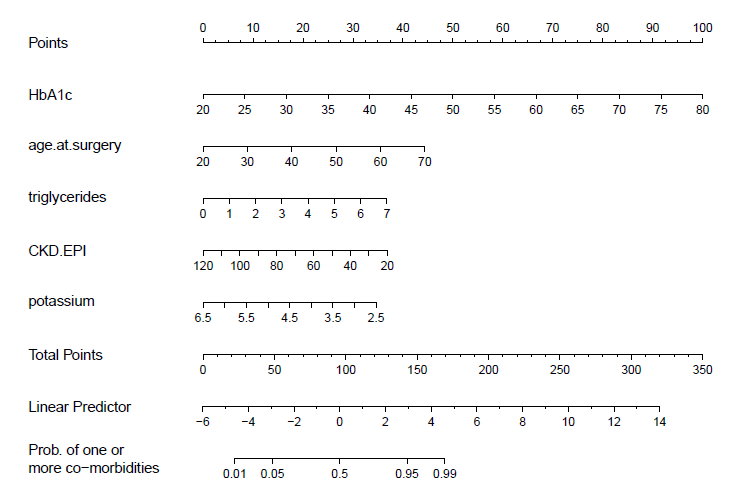
\includegraphics[scale=0.8]{BariatricNomogram.png}
		\caption{The nomogram that explained the created comorbidity severity score of bariatric patients.\cite{Deneer2017Thesis}}
		\label{fig:BariatricNomogram}
	\end{figure}
	
	
	\subsection{Automated Machine Learning}
	\label{subsec:AutomatedMachineLearning}
	
	% History autoML
	Before automated machine learning (autoML) existed, a dataset was mined by hand. First a preprocessing algorithm was chosen and used to prepare the data. Next a (machine learning) algorithm was chosen to mine the desired results out of the data. At last the hyperparameters of the chosen algorithm were tuned to optimize the desired results. These three steps are vastly different and significant issues arise when combining these. Several ideas arose to combine the steps, called Combined Algorithm Selection and Hyperparameter optimization (CASH).\cite{thornton2013auto} After some time, when preprocessing was added in the mix as well, the name autoML was being used.\cite{Gijsbers2017Thesis} The first autoML approach tool was published as \texttt{Auto-WEKA} that focused on classification methods, spanning 2 ensemble methods, 10 meta-methods, 27 base classifiers and their hyperparameter settings.\cite{thornton2013auto} An upgrade was published that added regression and parallellism.\cite{kotthoff2016auto}   
	
	% Introduction to pipelines
	As explained shortly before, to go from data and results several steps must be taken: Preprocessing, algorithm selection and hyperparameter optimization. This sequencing is called a machine learning pipeline. Such a pipeline can consists of zero, one or multiple preprocessing steps for data preparation, can be one of many different machine learning algorithms which on their part have wide ranges for multiple hyperparameters. The explosion of possible pipelines makes it hard to choose the right one. Knowing successful combinations is useful, however every data set has different features that ask for different pipelines. \cite{Gijsbers2017Thesis}
	
	% Introduction autoML
	AutoML tires to find the best machine learning pipelines to compute which algorithms must be selected, combined with tuning the hyperparameters and preprocessing. This algorithm selection usually is done in a meta-learning approach, which focuses on finding how the machine learning algorithms perform for a task interval. Hyperparameter optimization has challenges on his own to find the right ones and there are many different approaches to tackle preprocessing. All of these are discussed in their own subsection to briefly explain them.	
	
	
	\subsubsection{Meta-Learning}
	\label{subsubsec:Meta-Learning}
	
	% Introduction meta-learning
	Machine learning algorithms show different behaviour for different tasks. Meta-learning tries to find out how their performance changes between those tasks (Figure \ref{fig:Meta-LearningLayout}). It tries to link the algorithm with data sets it would do good for and tries to find which hyperparameters give a good performance. In combination with the machine learning pipelines, meta-learning would try to find the best ones available. Since not only algorithms must be selected, but also hyperparameters must be optimized and preprocessing must be done, the time and space needed for meta-learning explodes. This can be lessened when removing bad pipelines and limiting the range of hyperparameters, machine learning- and preprocessing algorithms as much as possible. 

	\begin{figure}
		\label{fig:Meta-LearningLayout}
		\includegraphics[scale=1]{Meta-LearningLayout.png}[h!]
		\caption{A layout of how meta-learning works. 1. Data sets are collected. 2. Meta-data is computed for each dataset. 3. A meta-dataset is created and a meta-model is learned.\cite{Gijsbers2017Thesis}}
	\end{figure}
	
	% Meta-features
	Features of the meta-learning phenomenon are used to predict the performance. There are three types of these meta-features. The first type is simple, statistical and information-theoretic. They can be a basic feature of the data set, as well as a value after a statistical computation or a specific theoretical value. The second meta-feature type can be called landmarks. Landmarks give the performance of algorithms, how well they are doing with the given data set. The last meta-feature category is model-based. Specific characteristics of the used model can be used as meta-features as well.\cite{brazdil1994characterizing, vilalta2004using}

	% Meta-learners
	For using those meta-features in picking the best machine learning algorithm meta-learners can be used. Meta-learners are algorithms that choose between the possible choices. There are four ways of doing that. The first is plainly choosing the best algorithm in the set, this choice speeds up the process but is prone to being a bad choice. Second a subset of good algorithms can be chosen, which is slower, but has a higher chance to give a good outcome. Thirdly the algorithms can be ranked, which makes the chance of picking a good algorithm quicker starting at the top. Fourth is to use estimations of performance which gives information expectations over all algorithms.\cite{brazdil2009development}

	\subsubsection{Hyperparameter Optimization}
	\label{subsubsec:Hyperparameter optimization}

	% Introduction to hyperparameters
	As discussed before, machine learning algorithms have hyperparameters. These type of parameters are very sensitive and can change the algorithm performance greatly, hence the hyper- prefix. These hyperparameters can be nonlinear and nonconvex which results in it being hard to find the optimal value. They are many different variable types of hyperparameters, which makes standardizing optimization hard. They can also be dependent on each other and therefore have useless combinations. At last they can change the computation time drastically for a minor change in parameter.\cite{claesen2015hyperparameter}

	% Ways to find the right parameters
	There are several approaches to find the right values for the hyperparameters. Three approaches will be discussed. At first there is grid search, that checks all possible combinations for hyperparameters on a predefined interval. This approach does effectively check the complete area the optimal solution can be in, however it also takes much computational time due to the combinatorial explosion principle.\cite{hsu2003practical} A second approach is the random search, when values are chosen for each hyperparameter at random. It is proven that this search is better in an empirical and theoretical way, due changing some hyperparameters hardly making any difference.\cite{bergstra2012random} 
	
	% Bayesan optimization
	A more advanced way of optimizing hyperparameters is Bayesian Optimisation. This hyperparameter optimization approach tries to use earlier results to find the best possible location for the hyperparameters to be optimized. At the start, with random sampling several sample points are measured. An acquisition function, with the input from earlier samples, which combination of hyperparameters should be tested next. It balances between trying to explore areas with good performance and trying to explore bigger areas for possible other good areas.\cite{snoek2012practical} The three optimization techniques are shown together to explain the difference (Figure \ref{fig:HyperparameterOptimization}).
	
	\begin{figure}
		\label{fig:HyperparameterOptimization}
		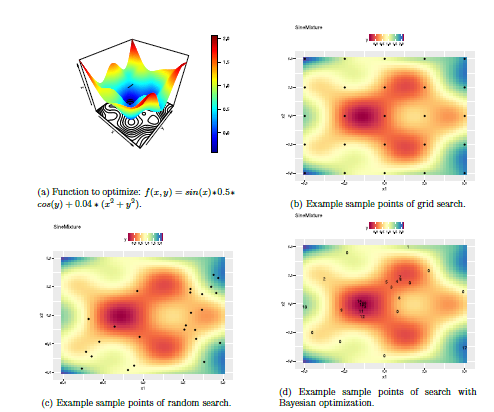
\includegraphics[scale=0.8]{HyperparameterOptimization.png}[H!]
		\caption{Examples of the three explained hyperparameter optimization techniques. The numbers in the bayesan optimization show the iteration of sampling.\cite{Gijsbers2017Thesis}}
	\end{figure}
	
	\subsubsection{Preprocessing}
	\label{subsubsec:Preprocessing}
	
	% Introduction preprocessing
 	Preprocessing is one of the three aspects of autoML. Whereas the goal is important when choosing a type of machine learning algorithm, preprocessing algorithms always need to be fine-tuned for the available data set, as every set is different. Data sets, and specially biomedical ones for this project, have specific challenges that can be solved using preprocessing (subsection \ref{subsec:BiomedicalData}). These challenges can be classified in two regions. The first one is about problems with the data, Tye second one is data preparation.\cite{famili1997data}
 	
 	% Too much data
 	From a preprocessing point of view, there can be three different types of problems with data (Figure \ref{fig:DataPreprocessing}). The first problem is that there is too much data. The data can be noisy, irrelevant, too big, different types of data can be present and feature extraction still has to be done. The data for this project is an example for noisy data (subsection \ref{subsec:BiomedicalData}), as 5\% of the data is estimated to be wrong.
 	
 	% Too little data
 	A second type is the opposite of having too much data. There can also be too little data. Values of an attribute or complete attributes can be absent from the data. The number of data points can also be very low. For the example data set, there were many cases where attributes were missing.
 	
 	% Fractured data
	A third problem with the data can be that it is fractured. Multiple separate data sets can be incompatible, come from multiple sources or are on different processing levels. When taking the bariatric data as an example, it stems from two different data sets. A challenge is to combine these two as one data set, as one, while they are not specifically made for that.
 	
	% Data preprocessing techniques/Data transofmration
	To tackle those three data problems, again three types of techniques can be used. At first data can be transformed to become more usable. The most important transformation is noise removal. It can be removed with smoothing function\cite{somorjai2004data, karagiannis2011noise}, or a more advanced machine learning technique to also detect it.\cite{gamberger2000noise}
 	
 	% Information gathering
 	A second preprocessing technique is gathering data if needed. Data selection is important, as it could be that not all data is as relevant as all the other data. Important techniques to be mentioned are principal component analysis, that checks the relevance for every feature in the data set.\cite{duszak1994using} 
 	
 	% Generation of new information
 	At last new information can be generated, if needed. This can be done by simulation or by adding new features. Data points can be fused to become a new point. This way more data is available for data analysis. Also when values are missing, several techniques can be used for value imputation. Extrapolation can be done, using regression to estimate its value. Other methods are based on nearest neighborhood frameworks.\cite{zhu2011missing} 
 	
 	\begin{figure}[h!]
 		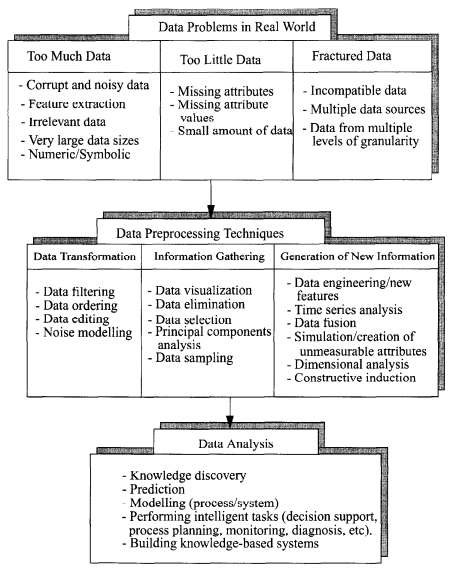
\includegraphics[scale=1]{DataPreprocessing.png}
 		\caption{A schema that shows the process of preprocessing.\cite{famili1997data}}
 		\label{fig:DataPreprocessing}
 	\end{figure}
 	
 	% Rawness challenges
 	Aside from data problems, another reason for preprocessing can be present.\cite{famili1997data} Data can also be very raw. STo reach a certain goal, a data set has the necessary iformation, but only indirectly. An example would be hypertension. To know if someone has hypertension, its blood pressure must be measured and checked if that value is high enough. this preprocessing is highly data set specific, as computers do not know the specifications of blood pressure for someone having hypertension. 
 	
	\subsection{Tree-based Pipeline Optimization Tool}
	\label{subsec:TPOT}
	
	% Introduction TPOT
	A tool that implements autoML is tree-based pipeline optimization tool (TPOT). It uses the machine learning pipelines and evolutionary optimization to find the best solution for every data set. This evolutionary optimization is done by genetic programming. Genetic programming evolves possible solutions to find a better solution. This evolution is done by first evaluating them and selecting the best ones to continue to the next generation. Then both crossovers between and mutations on possible solutions are performed. After that again evaluation and selection, followed by crossovers and mutations, take place a number of times until a certain quality is found, time has run out or another ending condition has been met.
	
	% TPOT layout
	TPOT makes use of this genetic programming with using the machine learning pipelines in a tree (Figure \ref{fig:MachineLearningPipeline}). TPOT consists of preprocessing and machine learning algorithms, that form the backbone of the pipelines. Their hyperparameters and the data set are the variables. TPOT makes mostly use of the machine learning and preprocessing algorithms of skikit-learn from Python in which it is also written.
	
	\begin{figure}[h!]
		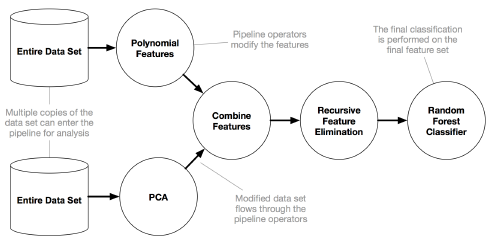
\includegraphics[scale=1]{MachineLearningPipeline.png}
		\caption{An example of a machine learning pipeline in TPOT. It only shows the primitive algorithms and not hyperparameter terminals. At the root is the machine learning algorithm.\cite{Gijsbers2017Thesis}}
		\label{fig:MachineLearningPipeline}
	\end{figure}

	% TPOT mutation operators
	TPOT has three different types of mutations within one pipeline.The first one is insertion, inserting a primitive somewhere in the tree. An example would be the insertion of an additional preprocessing algorithm. The second one is replacement, which replaces a random terminal. It can for example change a binary hyper parameter from true to false. The third one is shrinking. A primitive is replaced by a terminal. For example a preprocessing step can be replaced by just raw data. This different mutations can all be seen visually (Figure \ref{fig:TPOTMutations})
	
	\begin{figure}[h!]
		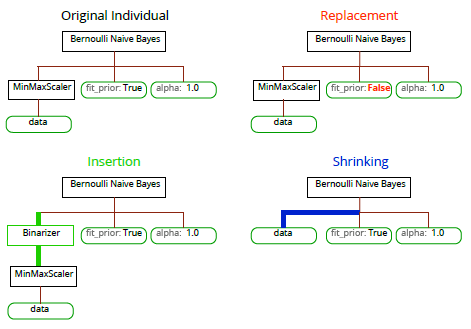
\includegraphics[scale=1]{TPOTMutations.png}
		\caption{Examples of the three mutations in the TPOT algorithm: insertion, replacement and shrinking.\cite{Gijsbers2017Thesis}}
		\label{fig:TPOTMutations}
	\end{figure}
	
	% Crossover
	TPOT also focuses on mutations between two pipelines through the means of crossovers. Between two pipelines, sub-trees and primitives can be changed, given that the both pipelines remain valid (Figure \ref{fig:TPOTCrossover}). Every time a crossover is performed, two separate pipelines are used and changed, creating two new ones.
	
	\begin{figure}[h!]
		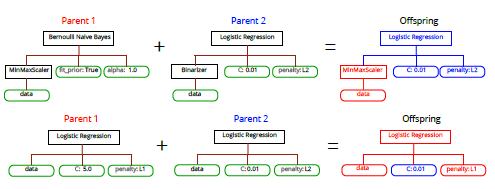
\includegraphics[scale=1]{TPOTCrossover.png}
		\caption{An example of a TPOT crossover\cite{Gijsbers2017Thesis}}
		\label{fig:TPOTCrossover}
	\end{figure}
	
	% Biomedical preprocessing
	Comparing the possibilities from TPOT and the challenges in biomedical data, it seems that TPOT has some implementations to tackle them. It has several different scalers (StandardScaler, RobustScaler, MinMaxScaler) to tackle feature heterogeneity between different data sets and errors. It also has some feature selection operators to tackle errors (VarianceThreshold, SelectKBest, SelectPercentile). For missing values, the algorithm imputes the median as estimation for the missing value.
	
	\section{Research Question}
	
	%Introduction research question
	TPOT has shown to give promising results for several different data sets.\cite{Gijsbers2017Thesis} For this project the focus will be on biomedical data sets (subsection \ref{subsec:BiomedicalData}) and how it handles specific problems in these data sets. An example data set (subsection \ref{subsec:BariatricDataSet}) is taken for analysis and to create suggestions for future extensions of TPOT. The research question for TPOT will be the following.\\
	
	How does TPOT perform on specific biomedical data set problems and how can it be improved on them?\\
	
	% Hypothesis
	Knowing that some algorithms exist to tackle the problems with biomedical data sets, the first step should be to find out whether all problems can already be tackled by TPOT. This seems the case for fractured data and errors in the data, both challenges seem to have some way to be handled. Missing values however do not seem to be targeted. There are no ways to have value imputation and the only way this seems to be tackled is by giving it the median value. It seems improvement on that part would be beneficial and examples such as extrapolation and nearest neighbour algorithms seem good approach to tackle that.
	
	\bibliography{../References/Citings} 
	\bibliographystyle{ieeetr}
	
\end{document}
\